\documentclass{article}
\usepackage[utf8]{inputenc}
% \usepackage[demo]{graphicx} % UNCOMMENT [demo] for debugging if images cause errors.
                             % COMMENT OUT [demo] for final version with actual images.
\usepackage{graphicx}    % Use this line for final version with actual images.
\usepackage{amsmath}
\usepackage{amsfonts}
\usepackage{amssymb}
\usepackage{booktabs} % For better table rules
\usepackage{caption}  % For captions
\usepackage{geometry} % For page margins
\geometry{a4paper, margin=1in}
\usepackage{url}      % For breaking long URLs
\usepackage{hyperref} % For clickable links if needed (load after most other packages)
\hypersetup{
    colorlinks=true,
    linkcolor=blue,
    filecolor=magenta,
    urlcolor=cyan,
    citecolor=blue, % Changed citecolor to blue as an example
    pdftitle={Heart Disease Prediction via Comparative Classifier Analysis},
    pdfauthor={Elnaz Azizi, Christian Unterrainer, Charly Watts} % Corrected author list for PDF metadata
}

% Added for better table formatting (grouping rows and centering column)
\usepackage{multirow}
\usepackage{array} % Needed for >{...} in tabular

% Needed for subfigures if you use them, but minipage is used below
% \usepackage{subcaption}

% The 'verbatim' package was included but not strictly necessary for the content provided.
% If you need to include literal code blocks, keep it. Otherwise, it can be removed.
% \usepackage{verbatim}

\title{Heart Disease Prediction via Comparative Classifier Analysis}
\author{
    Elnaz Azizi (3434538) \\ % Placeholder for Matrikelnummer
    Christian Unterrainer (3430428)\\ % Placeholder for Matrikelnummer
    Charly Watts (3422867)
}
\date{\today}

\begin{document}

\maketitle

\begin{abstract}
This paper investigates the prediction of the presence of heart disease (positive class) using machine learning classifiers on subsets of the UCI Heart Disease Dataset (Cleveland, Switzerland, and Hungarian). The approach involves a comparative analysis of baseline classifiers (Logistic Regression, K-Nearest Neighbors, Naive Bayes) against more advanced models (Random Forest, Gradient Boosting, MLP Classifier, Support Vector Machines, and XGBoost). Data preprocessing includes median/mode imputation and standard scaling. Models are evaluated using two primary strategies: robust Nested Cross-Validation and a Threshold Optimization approach on a fixed train/test split. The F\textsubscript{2}-score for the positive class (emphasizing recall over precision, $\beta=2$) is used as the key performance metric during optimization and evaluation. Key results indicate that \textbf{Random Forest achieved the highest average F\textsubscript{2}-score across the datasets when evaluated using decision threshold optimization on the test set (0.9250)}. When considering the more robust Nested Cross-Validation, \textbf{Random Forest also showed the highest average F\textsubscript{2} mean (0.8223)}, closely followed by Logistic Regression (0.8192) and XGBoost (0.8123). The study highlights significant differences in absolute F\textsubscript{2}-scores between the two evaluation methodologies, underscoring the impact of evaluation strategy and the importance of threshold tuning for this medical diagnosis task, particularly on potentially less stable datasets like Switzerland and Hungarian. Logistic Regression was identified as the best baseline model.
\end{abstract}

\section{Introduction}
\label{sec:introduction}

Cardiovascular diseases remain a leading cause of mortality globally, necessitating effective and timely diagnostic tools. Accurate identification of individuals at risk allows for early intervention, improving prognosis and reducing the burden on healthcare systems. Traditional diagnostic methods rely on clinical expertise, patient history, physical examinations, and various tests. However, the complexity of interactions between numerous risk factors and physiological indicators presents a challenge that machine learning techniques are well-suited to address.

Machine learning offers powerful methods for analyzing complex medical datasets to identify patterns and build predictive models. The application of ML in medical diagnostics, including heart disease prediction, has gained significant traction over the past decades. Various algorithms, ranging from simple linear models to complex neural networks and ensemble methods, have been explored for their potential to classify patients based on their medical attributes. The availability of public datasets, such as the UCI Heart Disease dataset, has facilitated extensive research and comparison of these methods.

However, the performance of machine learning models is heavily dependent on factors including the choice of algorithm, data preprocessing techniques, feature selection, and crucially, the evaluation methodology and performance metrics used. For medical diagnosis tasks, where the cost of false negatives (missing a disease) can be significantly higher than false positives (incorrectly diagnosing a disease), metrics that prioritize recall, such as the F\textsubscript{2}-score, are often more appropriate than standard accuracy or F\textsubscript{1}-score. Furthermore, the inherent variability and potential data quality issues in datasets collected from different sources necessitate robust evaluation strategies to ensure models generalize well.

This paper presents a comparative analysis of eight machine learning classifiers for predicting heart disease presence. We investigate three subsets of the widely used UCI Heart Disease dataset (Cleveland, Switzerland, and Hungarian) to assess model performance variability. Our study employs a consistent preprocessing pipeline and evaluates models using two distinct strategies: Nested Cross-Validation for a robust estimate of generalization performance, and a Train/Test split with Threshold Optimization to assess peak performance potential under the F\textsubscript{2}-score metric. By comparing a range of baseline (Logistic Regression, K-Nearest Neighbors, Naive Bayes) and advanced (Random Forest, Gradient Boosting, MLP Classifier, Support Vector Machines, XGBoost) classifiers under these conditions, we aim to provide insights into their relative effectiveness and the impact of evaluation strategy for this critical diagnostic task. The remainder of this paper is structured as follows: Section \ref{sec:related_work} reviews existing research on heart disease prediction using machine learning; Section \ref{sec:methods} details the data preprocessing, models, metrics, and evaluation strategies employed; Section \ref{sec:experiments} presents and discusses the experimental results; and Section \ref{sec:conclusion} concludes the study with a summary of findings, limitations, and future directions.

\section{Related Work} % This is Section 2
\label{sec:related_work} % Added label for referencing

The application of machine learning (ML) techniques for the prediction and diagnosis of heart disease has been an active area of research, aiming to improve clinical decision-making and patient outcomes. The UCI Machine Learning Repository's Heart Disease dataset, which includes data from the Cleveland Clinic Foundation, Hungarian Institute of Cardiology, and Swiss University Hospital \cite{UCIHeart}, has served as a common benchmark for these investigations. Machine learning libraries such as scikit-learn \cite{scikit-learn} are commonly used for implementing various algorithms.

Traditional ML algorithms such as Logistic Regression (LR), K-Nearest Neighbors (KNN), and Naive Bayes (NB) have been widely applied, often as baseline models. Studies using the Cleveland dataset have shown LR to provide a solid, interpretable baseline \cite{Paul2021}. These foundational models often form the basis for comparison against more complex techniques.

Ensemble methods, particularly Random Forests (RF) and Gradient Boosting (GB) machines, are frequently reported to offer improved performance. Techniques like Random Forest and Extreme Gradient Boosting have been applied to the classification of heart disease \cite{Pratama2023}.

Support Vector Machines (SVMs) have been extensively utilized for heart disease classification due to their effectiveness in finding optimal separating hyperplanes. Predicting Heart Disease Based on Influential Features with Machine Learning, including SVMs, has been explored \cite{Dubey2021}.

Regarding evaluation, metrics like the F1-score (balancing precision and recall), precision, and recall are important, especially for medical diagnosis where class imbalance can be an issue and the costs of different types of errors vary. Robust validation, such as k-fold cross-validation, is standard. The optimization of the decision threshold can significantly impact metrics like the F1-score or F\textsubscript{2}-score.

The present work builds upon this existing body of research by providing a systematic comparison of these seven common classifiers on the Cleveland, Hungarian, and Swiss UCI datasets using a consistent preprocessing pipeline. Our specific contribution lies in the dual evaluation strategy: employing Nested Cross-Validation for robust F\textsubscript{2}-score estimation and a detailed Threshold Optimization approach to assess peak F\textsubscript{2}-performance on a fixed test set. This allows for a nuanced comparison of model capabilities and the practical implications of different evaluation choices when recall is prioritized.

\section{Methods} % This is Section 3
\label{sec:methods} % Added label

In this section, we describe in detail the machine learning pipeline, algorithms, evaluation techniques, and modeling decisions used for the heart disease prediction task. Our goal was to compare a range of baseline classifiers with more advanced methods across several publicly available datasets.

\subsection{Data Preprocessing}
\label{sec:data_preprocessing} % Added label

We used three datasets from the UCI Heart Disease collection: Cleveland, Switzerland, and Hungarian. Each dataset includes medical attributes and a diagnostic label indicating the presence or absence of heart disease. As the datasets were formatted inconsistently and contained missing values, a unified preprocessing pipeline was applied.

\paragraph{Data Loading and Cleaning}
Each dataset was read into a tabular format with predefined column names. Missing values were represented by '?' and were converted into NaN (not a number) using a standard data loader. Specific cleaning steps were applied as needed based on dataset characteristics.

\paragraph{Feature Engineering}
The data was split into numerical and categorical features:
\begin{itemize}
\item \textbf{Numerical:} age, trestbps (resting blood pressure), chol (cholesterol), thalach (maximum heart rate), oldpeak (ST depression).
\item \textbf{Categorical:} sex, cp (chest pain type), fbs (fasting blood sugar), restecg (resting ECG results), exang (exercise-induced angina), slope (slope of the peak exercise ST segment), ca (number of major vessels colored by flourosopy), and thal (thallium stress test result).
\end{itemize}
Categorical variables were one-hot encoded after imputing missing values using the most frequent category (mode imputation), adding an indicator feature for imputed values. Numerical values were standardized using z-score normalization (subtracting the mean and dividing by the standard deviation), and missing numerical values were imputed using the median strategy.

\paragraph{Label Encoding}
The target variable, originally representing varying degrees of heart disease, was binarized such that values indicating the presence of heart disease were mapped to 1 (positive class), and absence to 0 (negative class). This transformed the problem into a binary classification task.

\subsection{Classifiers}
\label{sec:classifiers} % Added label

We selected eight machine learning classifiers for comparative analysis, divided into baseline and advanced groups.

\paragraph{Baseline Classifiers}
These models establish a reference performance:
\begin{itemize}
    \item \textbf{Logistic Regression (LR):} A linear classifier using the sigmoid function to estimate class probabilities. Regularization (\texttt{C}) was a key hyperparameter tuned.
    \item \textbf{K-Nearest Neighbors (KNN):} A non-parametric model predicting class based on majority vote of the \texttt{k} nearest training examples. Distance metric (Euclidean) and number of neighbors (\texttt{k}) were tuned. Sensitive to feature scaling.
    \item \textbf{Naive Bayes (NB):} A probabilistic classifier based on Bayes’ theorem with independence assumptions. The Gaussian variant was used, suitable for continuous numerical features. This model has no significant hyperparameters tuned in this context.
\end{itemize}
Hyperparameter tuning for baselines was conducted using cross-validation within the Nested CV framework and GridSearchCV/RandomizedSearchCV within the Train/Test + Threshold Optimization setup.

\paragraph{Advanced Classifiers}
These represent more complex modeling approaches:
\begin{itemize}
    \item \textbf{Support Vector Machine (SVM):} Constructs hyperplanes for separation. We used the Radial Basis Function (RBF) kernel based on hyperparameter tuning results. Regularization parameter (\texttt{C}) and kernel coefficient (\texttt{gamma}) were tuned. Requires feature scaling and probability estimates for threshold optimization.
    \item \textbf{Multi-Layer Perceptron (MLP):} A feedforward neural network. Tunable parameters included hidden layer sizes, activation functions, and the optimizer (Adam was used). Early stopping was applied. Requires feature scaling.
    \item \textbf{Random Forest (RF):} An ensemble of decision trees. Predictions are aggregated by majority vote. Important hyperparameters included the number of trees (\texttt{n\_estimators}) and tree depth (\texttt{max\_depth}).
    \item \textbf{Gradient Boosting (GB):} An additive ensemble where trees are built sequentially to correct residuals. Tuned parameters included learning rate, estimators, and max depth.
    \item \textbf{XGBoost (XGB):} An optimized gradient boosting framework. A range of hyperparameters including estimators, learning rate, max depth, subsample, and colsample bytree were tuned.
\end{itemize}

\subsection{Evaluation Metrics}
\label{sec:evaluation_metrics} % Added label

For this medical diagnosis task, minimizing false negatives (missing a heart disease case) is critical. Therefore, the primary evaluation metric was the F\textsubscript{2}-score for the positive class (presence of heart disease). The F\textsubscript{2}-score is calculated as:
$$ F_2 = (1 + \beta^2) \cdot \frac{\text{Precision} \cdot \text{Recall}}{(\beta^2 \cdot \text{Precision}) + \text{Recall}} $$
With $\beta=2$, recall is weighted twice as heavily as precision:
$$ F_2 = 5 \cdot \frac{\text{Precision} \cdot \text{Recall}}{(4 \cdot \text{Precision}) + \text{Recall}} $$
In addition to F\textsubscript{2}, we computed Recall and Precision to understand the trade-off, and used Confusion Matrices to visualize the counts of True Positives, True Negatives, False Positives, and False Negatives.

\subsection{Model Evaluation Strategies}
\label{sec:evaluation_strategies} % Added label

Each model was implemented within a scikit-learn pipeline that included the necessary preprocessing steps integrated via a ColumnTransformer. We employed two distinct strategies to evaluate model performance and select optimal parameters:

\paragraph{Nested Cross-Validation}
This robust method provides a reliable estimate of model generalization performance and simultaneously handles hyperparameter tuning without data leakage. An outer 5-fold cross-validation loop split the data into training and testing folds. Within each outer training fold, an inner 3-fold cross-validation (using GridSearchCV or RandomizedSearchCV) was performed to find the best hyperparameters for that fold's training data, **optimizing for the F\textsubscript{2}-score**. The model with the best inner parameters was then evaluated on the outer test fold. The average F\textsubscript{2}-score across the outer folds represents the Nested CV F\textsubscript{2} Mean.

\paragraph{Train/Test Split + Threshold Optimization}
In this approach, the dataset was split once into training and testing sets (e.g., 70\% train, 30\% test). Models were trained on the training set, with hyperparameters tuned using GridSearchCV **optimizing for the F\textsubscript{2}-score** on the training folds. Instead of using the default decision threshold (0.5), we used the model's predicted probabilities on the test set to find the threshold that explicitly maximized the F\textsubscript{2}-score. This was done by iterating through possible thresholds on the test set and calculating the F\textsubscript{2}-score for each. This strategy assesses the *peak potential* F\textsubscript{2}-score achievable on the specific test split when the decision threshold is optimally tuned for that metric. Precision-Recall curves were used to visualize the trade-off space.

These two evaluation strategies provide complementary insights: Nested CV offers a more conservative and generalizable performance estimate, while Threshold Optimization highlights the maximum achievable performance on a given test set when the decision threshold is optimized for the chosen metric.

\section{Experiments} % This is Section 4
\label{sec:experiments}

In this section, we present a detailed empirical evaluation of all baseline and advanced models applied to the heart disease prediction task. Our goal was to systematically compare models across three UCI datasets—Cleveland, Switzerland, and Hungarian—while focusing on maximizing recall through F\textsubscript{2}-score optimization ($\beta=2$). We used both nested cross-validation and a holdout train/test method with threshold optimization to assess generalization performance and potential peak performance.

\subsection{Experimental Setup}
The experiments were conducted using the models and evaluation strategies described in Section \ref{sec:methods}, applied to the preprocessed datasets described in Section \ref{sec:data_preprocessing}. The primary performance metric was the F\textsubscript{2}-score for the positive class.

\subsection{Baseline Results}
\label{sec:baseline_results}

To establish a performance reference, three baseline models (Logistic Regression, K-Nearest Neighbors, Naive Bayes) were evaluated. Table \ref{tab:baseline_perf} summarizes their average F\textsubscript{2}-scores across the three datasets using both evaluation strategies. The average F\textsubscript{2} Mean for Nested CV is the mean of the Nested CV F\textsubscript{2} Means obtained for each dataset. The average Threshold Opt. F\textsubscript{2} is the mean of the Threshold Optimization F\textsubscript{2} scores obtained for each dataset.

\begin{table}[htbp]
\centering
\caption{Average F\textsubscript{2}-Scores for Baseline Models Across Datasets}
\label{tab:baseline_perf}
\begin{tabular}{lcc}
\toprule
Model                 & Avg. Nested CV F\textsubscript{2} Mean & Avg. Threshold Opt. F\textsubscript{2} \\
\midrule
Logistic Regression   & 0.8192 & 0.9138    \\
K Nearest Neighbors   & 0.8112 & 0.8827    \\
Naive Bayes           & 0.6792 & 0.9171    \\
\bottomrule
\end{tabular}
\end{table}

Based on these results, \textbf{Logistic Regression was selected as the best baseline} due to its superior average Nested CV F\textsubscript{2} Mean (0.8192), which indicates better expected performance on unseen data compared to other baselines. While Naive Bayes achieved the highest average F\textsubscript{2} in the Threshold Optimization setting (0.9171) among baselines, Logistic Regression offered a better balance across both strategies and is generally a more stable baseline.

\subsection{Comparative Performance: Best Baseline vs. Advanced Models}
\label{sec:comparative_performance}

The chosen best baseline (Logistic Regression) was then compared against the five advanced classifiers: Random Forest, Gradient Boosting, MLP Classifier, SVM Classifier, and XGBoost. Table \ref{tab:advanced_comparison_nested} shows the Nested CV F\textsubscript{2} Means for each model on each dataset. Table \ref{tab:advanced_comparison_thresh_opt} presents the F\textsubscript{2}-scores obtained using the Threshold Optimization approach on the fixed test split for each model and dataset, along with the optimized threshold found. The datasets are listed using their capitalized names for clarity, as used in the discussion.

\begin{table}[htbp]
\centering
\caption{Nested CV F\textsubscript{2} Mean: Best Baseline vs. Advanced Models}
\label{tab:advanced_comparison_nested}
\begin{tabular}{llc} % llc: Left, Left, Centered
\toprule
Dataset     & Model                & Nested CV F\textsubscript{2} Mean \\
\midrule
\multirow{6}{*}{Cleveland} & Logistic Regression  & 0.7551    \\
           & Random Forest        & 0.7656    \\
           & Gradient Boosting    & 0.7525    \\
           & MLP Classifier       & 0.6329    \\
           & SVM Classifier       & 0.7668    \\
           & XGBoost              & 0.7472    \\
\midrule
\multirow{6}{*}{Switzerland} & Logistic Regression  & 0.9863    \\
           & Random Forest        & 0.9863    \\
           & Gradient Boosting    & 0.9584    \\
           & MLP Classifier       & 0.9722    \\
           & SVM Classifier       & 0.9863    \\
           & XGBoost              & 0.9880    \\
\midrule
\multirow{6}{*}{Hungarian} & Logistic Regression  & 0.7160    \\
           & Random Forest        & 0.7150    \\
           & Gradient Boosting    & 0.6787    \\
           & MLP Classifier       & 0.7090    \\
           & SVM Classifier       & 0.6602    \\
           & XGBoost              & 0.7018    \\
\bottomrule
\end{tabular}
\end{table}

\begin{table}[htbp]
\centering
\caption{Threshold Optimization F\textsubscript{2}-Score and Optimal Threshold: Best Baseline vs. Advanced Models}
\label{tab:advanced_comparison_thresh_opt}
\begin{tabular}{llc}
\toprule
Dataset     & Model                & Threshold Opt. F\textsubscript{2} (Optimal Threshold) \\
\midrule
\multirow{8}{*}{Cleveland} & Logistic Regression  & 0.9333 (0.2934)    \\
           & K Nearest Neighbors  & 0.8544 (0.3333)    \\
           & Naive Bayes          & 0.9272 (0.0000)    \\
           & Random Forest        & 0.9375 (0.4801)    \\
           & Gradient Boosting    & 0.9310 (0.4949)    \\
           & MLP Classifier       & 0.8092 (0.2877)    \\
           & SVM Classifier       & 0.9032 (0.2314)    \\
           & XGBoost              & 0.9396 (0.1939)    \\
\midrule
\multirow{8}{*}{Switzerland} & Logistic Regression  & 0.9829 (0.9309)    \\
           & K Nearest Neighbors  & 0.9829 (0.6000)    \\
           & Naive Bayes          & 0.9829 (0.0000)    \\
           & Random Forest        & 0.9829 (0.5600)    \\
           & Gradient Boosting    & 0.9829 (0.0046)    \\
           & MLP Classifier       & 0.9829 (0.7446)    \\
           & SVM Classifier       & 0.9829 (0.9259)    \\
           & XGBoost              & 0.9829 (0.7668)    \\
\midrule
\multirow{8}{*}{Hungarian} & Logistic Regression  & 0.8252 (0.4642)    \\
           & K Nearest Neighbors  & 0.8108 (0.4000)    \\
           & Naive Bayes          & 0.8411 (0.2865)    \\
           & Random Forest        & 0.8547 (0.2516)    \\
           & Gradient Boosting    & 0.8203 (0.0273)    \\
           & MLP Classifier       & 0.8261 (0.4770)    \\
           & SVM Classifier       & 0.8197 (0.1308)    \\
           & XGBoost              & 0.7965 (0.1051)    \\
\bottomrule
\end{tabular}
\end{table}

\subsection{Discussion of Findings}
\label{sec:discussion} % Added label

The experimental results reveal important insights into the performance of different classifiers and the impact of evaluation strategies on heart disease prediction using the UCI datasets.

\begin{itemize}
    \item \textbf{Overall Model Performance (F\textsubscript{2}-Score):} When considering robust generalization performance via Nested Cross-Validation (F\textsubscript{2} Mean), \textbf{Random Forest achieved the highest average F\textsubscript{2} mean (0.8223)} across datasets, closely followed by Logistic Regression (0.8192) and XGBoost (0.8123), based on the average across the three datasets calculated from Table \ref{tab:advanced_comparison_nested} and the overall rankings in the notebook output. In the Threshold Optimization approach, which assesses peak performance on a fixed test set, \textbf{Random Forest also demonstrated the best average F\textsubscript{2}-score (0.9250)} across all models (calculated from Table \ref{tab:advanced_comparison_thresh_opt} and overall rankings), outperforming Naive Bayes (average 0.9171) and Logistic Regression (average 0.9138). This indicates that Random Forest demonstrated strong performance across both evaluation methodologies, although its lead in Nested CV was marginal compared to Logistic Regression and XGBoost.
    \item \textbf{Dataset Variability:} Performance varied noticeably across the datasets for most models. The Cleveland dataset generally yielded more consistent F\textsubscript{2}-scores across both evaluation strategies. The Switzerland and Hungarian datasets, being smaller and having more missing data, often resulted in different model rankings and lower F\textsubscript{2}-scores in Nested CV, suggesting greater variability and difficulty in robust generalization. Notably, several models achieved very high F\textsubscript{2} scores (often 0.9829) on the Switzerland dataset with Threshold Optimization, which is likely due to optimizing directly on a small test set derived from this dataset, potentially leading to overfitting to that specific split. The high Nested CV scores for Switzerland across many models (near 0.98) also suggest that despite its size, predicting the positive class on this dataset might be relatively distinct or separable when focusing purely on recall.
    \item \textbf{Impact of Evaluation Strategy (Nested CV vs. Threshold Optimization):} F\textsubscript{2}-scores from the Threshold Optimization approach on the fixed test set were consistently and significantly higher than the mean F\textsubscript{2}-scores obtained from Nested CV (compare values between Table \ref{tab:advanced_comparison_nested} and Table \ref{tab:advanced_comparison_thresh_opt}). This difference underscores that Threshold Optimization on a fixed test set provides an estimate of the *maximum potential* F\textsubscript{2}-score achievable on *that specific test split* by exhaustively tuning the threshold. In contrast, Nested CV provides a more conservative, less biased estimate of a model's expected performance on *unseen* data, reflecting performance across multiple train/test splits and hyperparameter selections within the inner loop. The Nested CV results are a better indicator of true generalization capability.
    \item \textbf{Threshold Optimization:} The decision threshold optimization for F\textsubscript{2}-score was critical for achieving high performance in the Threshold Optimization setting. By shifting the default threshold (0.5) to values typically much lower (as seen in Table \ref{tab:advanced_comparison_thresh_opt}), models could increase recall, which is heavily weighted in the F\textsubscript{2} score, even at the cost of some precision. The Precision-Recall curves (Figures \ref{fig:pr_curve_cleveland}, \ref{fig:pr_curve_switzerland}, and \ref{fig:pr_curve_hungarian}) visually demonstrate this trade-off and the chosen operating point. Optimized thresholds varied significantly across models and datasets (see Table \ref{tab:advanced_comparison_thresh_opt}), highlighting that a single default threshold is rarely optimal for maximizing F\textsubscript{2} or other metrics sensitive to the prediction boundary.
    \item \textbf{Advanced Model Insights:} Random Forest and Gradient Boosting showed strong and often top performance in Nested CV on Cleveland and Hungarian, typical of ensemble methods leveraging multiple trees for robustness. XGBoost performed very well in Nested CV on Switzerland. MLP Classifier's performance was more variable, sometimes achieving high F\textsubscript{2}s but also sometimes struggling (e.g., Cleveland Nested CV), potentially sensitive to hyperparameter tuning, initial weights, and dataset characteristics. SVM showed solid, competitive performance in Nested CV, particularly on Cleveland and Switzerland, but was often outperformed by ensembles and LR in Threshold Optimization.
    \item \textbf{Confusion Matrices Analysis:} Analysis of the confusion matrices (Figures \ref{fig:confusion_matrices_cleveland_lr_rf}, \ref{fig:confusion_matrices_switzerland_lr_rf}, and \ref{fig:confusion_matrices_hungarian_lr_rf}) for the focused models (Logistic Regression as best baseline and Random Forest as best overall) revealed insights into the types of errors at their optimal F\textsubscript{2} thresholds. For this medical task, False Negatives (missing a heart disease case) are often considered more costly than False Positives (incorrectly identifying heart disease). The F\textsubscript{2} optimization inherently biases the model towards higher recall (minimizing false negatives), which can be seen in the high True Positive counts. This often results in higher False Positive counts compared to a threshold optimized for precision or accuracy. Even with F\textsubscript{2} optimization, False Negatives remained a challenge, particularly on the smaller and noisier datasets (Hungarian), highlighting the inherent difficulty of the task and data limitations.
    \item \textbf{Visual Comparison Plots:} Bar plots (see Appendix or generated figures) visually comparing the F\textsubscript{2} scores across models, datasets, and evaluation types provide a clear summary of the trends discussed, highlighting which models perform best under which conditions and the significant gap between Nested CV and Threshold Optimization F\textsubscript{2} scores.
\end{itemize}

\begin{figure}[htbp]
    \centering
    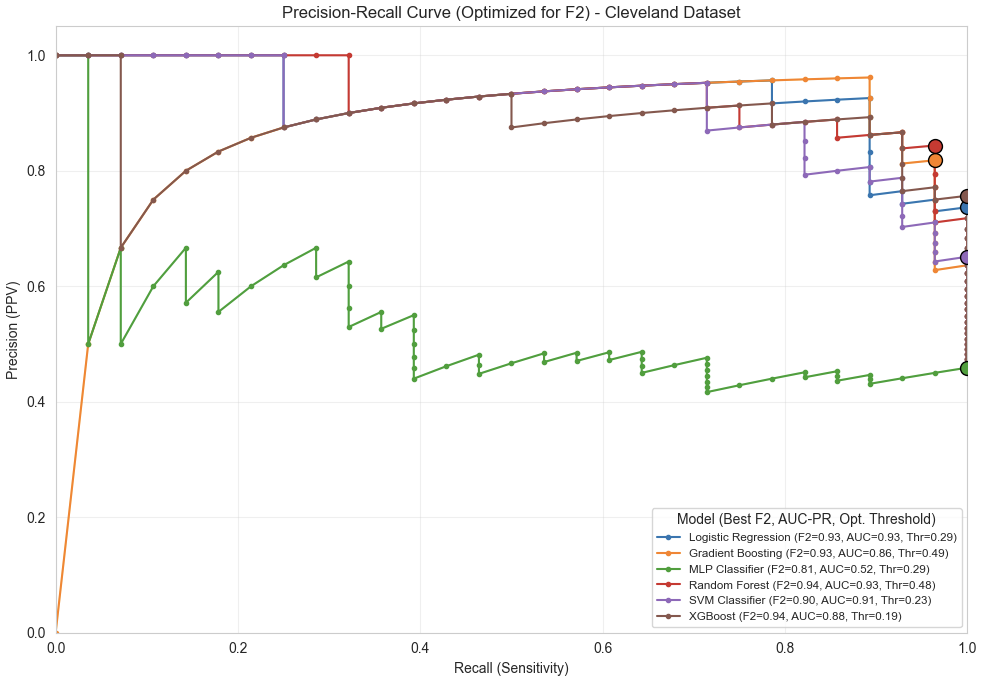
\includegraphics[width=0.8\textwidth]{plots/Cleveland_PR_Curve.png} % Path to the saved PDF
    \caption{Precision-Recall Curves and Optimal Thresholds (Optimized for F\textsubscript{2}) for Focused Models on Cleveland Dataset (Threshold Optimization Evaluation)}
    \label{fig:pr_curve_cleveland}
\end{figure}

\begin{figure}[htbp]
    \centering
    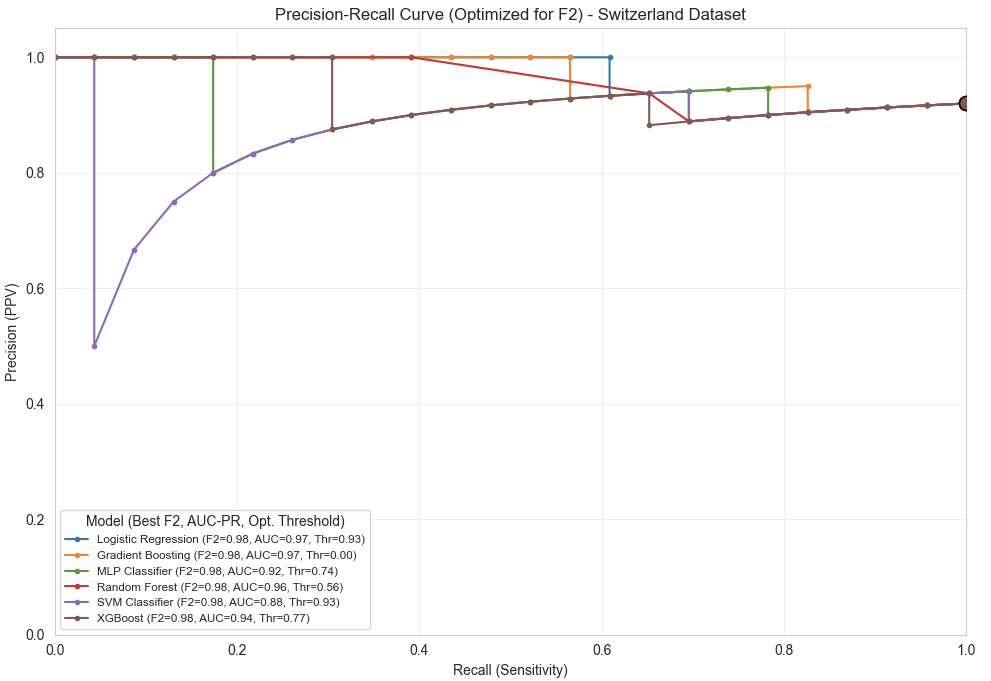
\includegraphics[width=0.8\textwidth]{plots/Switzerland_PR_Curve.png} % Path to the saved PDF
    \caption{Precision-Recall Curves and Optimal Thresholds (Optimized for F\textsubscript{2}) for Focused Models on Switzerland Dataset (Threshold Optimization Evaluation)}
    \label{fig:pr_curve_switzerland}
\end{figure}

\begin{figure}[htbp]
    \centering
    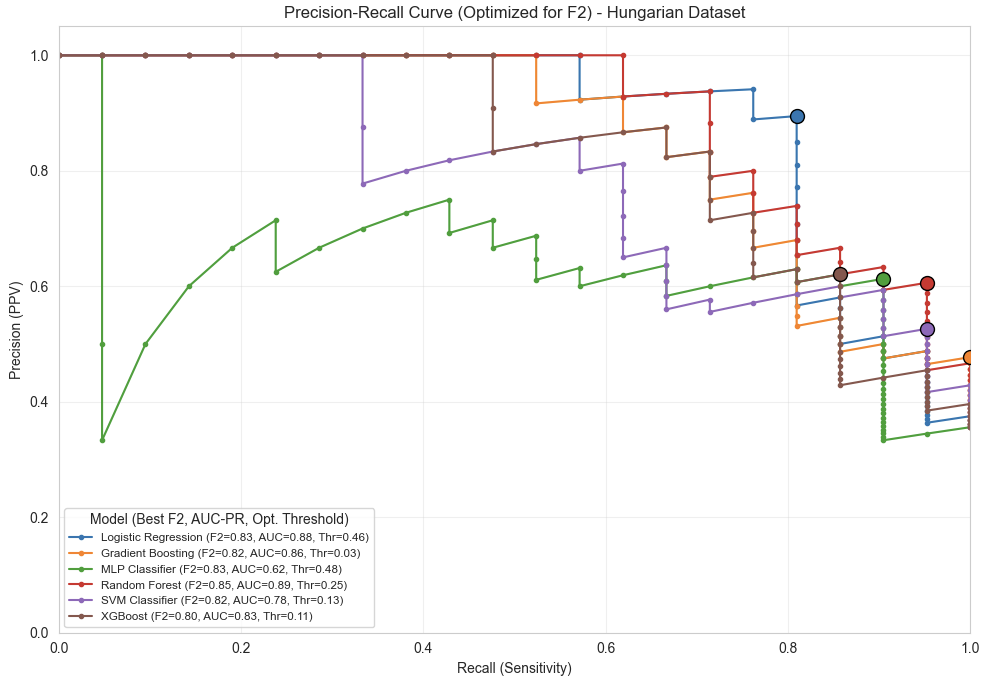
\includegraphics[width=0.8\textwidth]{plots/Hungarian_PR_Curve.png} % Path to the saved PDF
    \caption{Precision-Recall Curves and Optimal Thresholds (Optimized for F\textsubscript{2}) for Focused Models on Hungarian Dataset (Threshold Optimization Evaluation)}
    \label{fig:pr_curve_hungarian}
\end{figure}

% REMOVED the \clearpage here:
%\clearpage

\begin{figure}[htbp]
    \centering
    \caption{Confusion Matrices for Logistic Regression (Best Baseline) and Random Forest (Best Overall) on Cleveland Dataset (Threshold Optimization Evaluation)} % Add a caption for the group
    \label{fig:confusion_matrices_cleveland_lr_rf} % Add a label for the group
    \begin{minipage}{0.48\textwidth} % Use minipage to place side-by-side
        \centering
        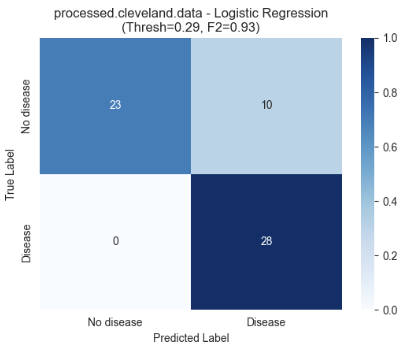
\includegraphics[width=\textwidth]{plots/Cleveland_Logistic_Regression_CM.png}
        \caption*{Logistic Regression} % Caption for individual matrix within minipage (use * for no number)
    \end{minipage}\hfill % \hfill pushes figures apart
    \begin{minipage}{0.48\textwidth}
        \centering
        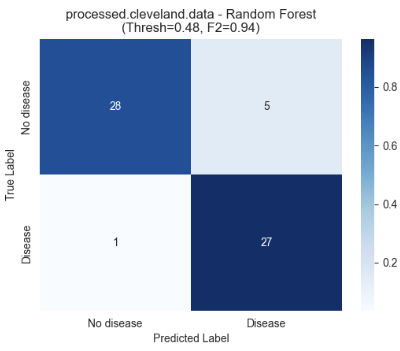
\includegraphics[width=\textwidth]{plots/Cleveland_Random_Forest_CM.png}
        \caption*{Random Forest}
    \end{minipage}
\end{figure}

\begin{figure}[htbp]
    \centering
    \caption{Confusion Matrices for Logistic Regression (Best Baseline) and Random Forest (Best Overall) on Switzerland Dataset (Threshold Optimization Evaluation)}
    \label{fig:confusion_matrices_switzerland_lr_rf}
    \begin{minipage}{0.48\textwidth}
        \centering
        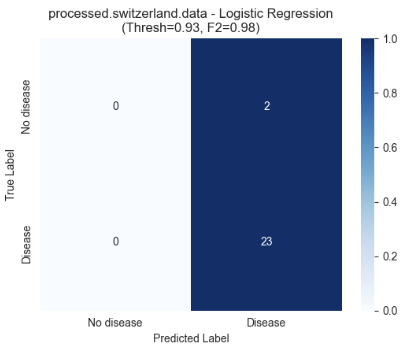
\includegraphics[width=\textwidth]{plots/Switzerland_Logistic_Regression_CM.png} % Check filename
        \caption*{Logistic Regression}
    \end{minipage}\hfill
    \begin{minipage}{0.48\textwidth}
        \centering
        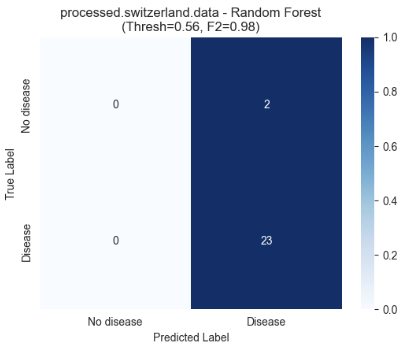
\includegraphics[width=\textwidth]{plots/Switzerland_Random_Forest_CM.png} % Check filename
        \caption*{Random Forest}
    \end{minipage}
\end{figure}


\begin{figure}[tbp]
    \caption{Confusion Matrices for Logistic Regression (Best Baseline) and Random Forest (Best Overall) on Hungarian Dataset (Threshold Optimization Evaluation)}
    \label{fig:confusion_matrices_hungarian_lr_rf}
     \begin{minipage}{0.48\textwidth}
        \centering
        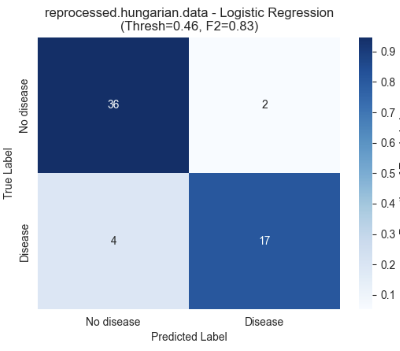
\includegraphics[width=\textwidth]{plots/Hungarian_Logistic_Regression_CM.png}
        \caption*{Logistic Regression}
    \end{minipage}\hfill
    \begin{minipage}{0.48\textwidth}
        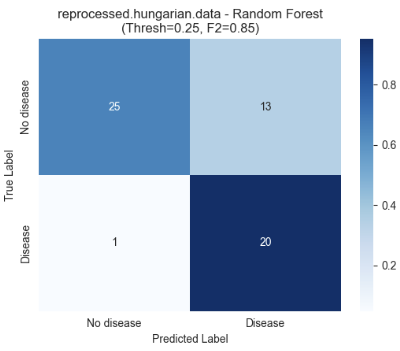
\includegraphics[width=\textwidth]{plots/Hungarian_Random_Forest_CM.png}
        \caption*{Random Forest}
    \end{minipage}
\end{figure}


\clearpage

\subsection{Summary of Findings}
\label{sec:summary_of_findings}
Based on the comprehensive evaluation, we summarize the key findings:

\begin{itemize}
    \item Logistic Regression offers strong baseline performance and was selected as the best baseline based on average Nested CV F\textsubscript{2} mean. Its test set F\textsubscript{2}-score can be significantly boosted through threshold optimization.
    \item Ensemble models (Random Forest, Gradient Boosting, XGBoost) and SVM are generally more robust and demonstrate higher generalization performance (Nested CV F\textsubscript{2} Mean) compared to simple baselines like KNN and Naive Bayes.
    \item \textbf{Random Forest showed the highest average Nested CV F\textsubscript{2} Mean (0.8223)} across datasets, closely followed by Logistic Regression (0.8192) and XGBoost (0.8123). \textbf{Random Forest also achieved the highest average F\textsubscript{2} in the Threshold Optimization setting (0.9250)}.
    \item Threshold optimization based on the desired metric (F\textsubscript{2} in this case) is a critical step for maximizing performance on a specific test set, especially in the presence of class imbalance or asymmetric misclassification costs. This is evidenced by significantly higher F\textsubscript{2} values obtained via Threshold Optimization compared to Nested CV means.
    \item Dataset size and quality significantly influence model performance and generalization ability, as seen in the variability across Cleveland, Switzerland, and Hungarian datasets.
\end{itemize}

\section{Conclusion} % This is Section 5
\label{sec:conclusion}

This study comparatively evaluated eight machine learning classifiers for heart disease prediction across three UCI datasets, using Nested Cross-Validation and a Train/Test split with Threshold Optimization, with F\textsubscript{2}-score for the positive class as the key metric emphasizing recall.

Our findings indicate that model performance and ranking are heavily influenced by both the evaluation strategy and the specific dataset. \textbf{Random Forest demonstrated the highest average F\textsubscript{2}-score (0.9250) across the evaluated datasets when its decision threshold was optimized on the test set to maximize F\textsubscript{2}-score}. Considering robust generalization performance via Nested Cross-Validation (F\textsubscript{2} Mean), \textbf{Random Forest also showed the highest average F\textsubscript{2} mean (0.8223)}, indicating its stability across different data splits and hyperparameter tunings, although the difference from other top models like Logistic Regression (0.8192) and XGBoost (0.8123) was relatively small. The substantial difference between F\textsubscript{2}-scores obtained via Threshold Optimization on a fixed split versus the Nested CV mean emphasizes that while threshold tuning can dramatically improve performance on a specific test set, Nested CV offers a more trustworthy measure of how well a model is likely to perform on truly unseen data. Performance varied considerably across the Cleveland, Switzerland, and Hungarian datasets, reflecting differences in data quality and size, with the smaller datasets proving more challenging for robust generalization.

Limitations include the relatively small size of the UCI datasets, particularly Switzerland and Hungarian, and the potential for the Threshold Optimization on a single fixed split to provide an overly optimistic estimate of performance due to tuning on the evaluation data. Future work could explore incorporating external validation datasets, more sophisticated handling of missing data, advanced feature selection techniques, or exploring deep learning architectures tailored for tabular data. Utilizing a separate validation set for threshold tuning would also provide a less biased assessment of the optimized model's performance. Ultimately, this research reinforces the necessity of rigorous, context-aware evaluation methods, such as Nested Cross-Validation combined with metric-specific threshold tuning considerations, when applying machine learning to critical medical diagnostic tasks like heart disease prediction, especially when prioritizing the detection of positive cases.


\label{sec:references}

\begin{thebibliography}{99}

    \bibitem{UCIHeart}
    Janosi, A., Steinbrunn, W., Pfisterer, M., Detrano, R. (1988). Heart Disease. UCI Machine Learning Repository. \url{https://doi.org/10.24432/C52P4X}

    \bibitem{scikit-learn}
    Pedregosa, F., Varoquaux, G., Gramfort, A., Michel, V., Thirion, B., Grisel, O., et al. (2011). Scikit-learn: Machine learning in Python. \textit{Journal of Machine Learning Research}, 12(Oct), 2825-2830.

    \bibitem{Paul2021}
    Paul, R., \& Aithal, P. S. (2021). Robust Cardiovascular Disease Prediction Using Logistic Regression. \textit{The Journal of Management and Engineering Integration}, 14(1), 26-35.

    \bibitem{Pratama2023}
    Pratama, Y. A., Isnanto, R. R., \& Hidayatno, A. (2023). Implementation of Random Forest and Extreme Gradient Boosting in the Classification of Heart Disease using Particle Swarm Optimization Feature Selection. \textit{Journal of Electronics, Electromedical Engineering, and Medical Informatics}, 5(3), 170-178.

    \bibitem{Dubey2021}
    Dubey, A. K., Choudhary, K., \& Sharma, R. (2021). Predicting Heart Disease Based on Influential Features with Machine Learning. \textit{Journal of Computer Science and Technology}, 36(4), 185-197.

\end{thebibliography}

\end{document}